% Chapter Template

\chapter{Theory} % Main chapter title

\label{Chapter2} % Change X to a consecutive number; for referencing this chapter elsewhere, use \ref{ChapterX}

\lhead{Chapter 2. \emph{Theory}} % Change X to a consecutive number; this is for the header on each page - perhaps a shortened title
\begin{doublespace}
Memristor studied in this thesis has a strip of PEDOT:PSS as a conductor. A drop of an electrolytic solution which has lithium and perchlorate ions is placed on top of this conducting strip. When the conductor has an applied potential, lithium ions inside the electrolyte solution migrate into PEDOT:PSS and modifiy its conductivity. Hole transport inside PEDOT:PSS as well as lithium and perchlorate movement is modeled using basic drift diffusion equations which are derived in the first part of this chapter. The second half of the chapter shows analytic solutions to drift diffusion equations which will be used to test the numerical methods derived in the following chapter.


\section{Carrier Transport Equations}
Drift diffusion equations, which are based on BTE, need to be solved in order to model the complex behaviour of the memristor. Drift-diffusion equations are derived by simplifying BTE equation via approximations. These simplifications dictate the limits of the drift-diffusion model and serve as guidelines for where this model can be used, therefore they need to be well understood.

Derivation of Boltzmann transport equation starts by stating that a distribution of charged particles can be defined by its position in space \textbf{r} and momentum \textbf{k} in time \textbf{t} using a probability distribution function f(k,r,t). This results in the most general form of Boltzmann transport equation.

\begin{equation}
\frac{d }{dt}f(k,r,t)=0
\end{equation}

This general form of BTE needs to be expanded and relevant physical equations need to be placed in to get an appropriate equation describing a specific problem or a device. 
Many different device simulators use some sort of approximation to BTE. In a semiconductor simulations they are commonly used for the movement and the density distribution of charge carriers such as holes (p) and electrons (n). 

After this brief introduction to BTE, rather than going through the mathematical derivation of the drift diffusion model, the approximations that are made along the process of derivation will be discussed in order to get a better insight on the model.  As a particle travels in a solid state device it collides with other particles as well as the atoms in the device. For drift-diffusion equations individual lattice scattering events or collisions are averaged and the particles have an average constant velocity under the effects of an electric field. This means that all the particles respond instantaneously to the changes in the electric field. The movement of the particles due to electric field is called the drift current. The relationship between drift velocity and the electric field is given by the following equation:

\begin{equation}
v=\mu E
\end{equation}

$\mu$ is called mobility constant and it determines the speed at which the particles are going to move when subject to an electric field. Drift current density can be derived based on drift velocity.

\begin{equation}
J_E=q n\mu E=q n v 
\end{equation}

Where q is the elementary charge and n is the electron density. In addition to the previous assumptions, it is assumed that the lattice is perfectly uniform, has a uniform temperature distribution and all the particles are close to the temperature of the lattice. Based on this assumption it is possible say that all the particles move due to thermal effects with the same thermal velocity ($v_{th}$) and mean free path ($l_f$). These quantities can be combined into one single coefficient called the diffusion constant. 

\begin{equation}
D=v_{th} \;l_f
\end{equation}

Drift and diffusion coefficients are related to each other via the Einstein relationship:

\begin{equation}
D=\frac{\mu k T}{q}
\end{equation}

Where k is the Boltzmann constant and T is the lattice temperature. The random thermally driven motion produces diffusion and results in a second term which contributes to carrier movement and it is called the diffusion current density.

\begin{equation}
J_D=qD\frac{dn}{dx}
\end{equation}

Unlike the drift current density, which is directly related to the carrier density, diffusion current density is related to the carrier density's first order derivative in space. Combining these two terms results in the following the current density equation for electrons in one dimension.

\begin{equation}
\vec{J_n^x}=q \mu_{n} n \vec{E_x}+qD_{n} \frac{dn}{dx} 
\label{cdenn}
\end{equation}

This equation can be easily extended to other dimensions by simply using the appropriate terms.

\begin{equation}
\vec{J_n^y}=q \mu_{n} n \vec{E_y}+qD_{n} \frac{dn}{dy} 
\end{equation}

Current density equations can be used for both positively and negatively charged particles by changing the sign of the diffusion current density.

\begin{equation}
\vec{J_p^x}=q \mu_{p} p \vec{E_x}-qD_{p} \frac{dp}{dx} 
\label{cdenp}
\end{equation}
Anisotropic drift and diffusion coefficients can be handled with ease by using different coefficients for different directions. Also mobility and diffusivity can be a function of any variable such as position or temperature. This is a useful property for a memristor simulation since hole mobility depends on lithium density in the PEDOT:PSS at any given position. 

Current density equations by themselves are not enough to solve this time dependent problem. It is necessary to account for the movement of charge over time which is captured in the continuity equation. It is basically a statement of conservation of particle density over time. The change in the amount of carriers over time in a particular area must be equal to the difference in current density over the same area. Additionally the amount of charge can change due to generation-recombination of charged particles. The continuity is captured by the equations:


\begin{equation}
\frac{\partial n}{\partial t}=\frac{1}{q}\nabla \cdot \vec{J_n}+U_{n}
\label{conn}
\end{equation}

\begin{equation}
\frac{\partial p}{\partial t}=-\frac{1}{q}\nabla \cdot \vec{J_p}+U_{p}
\label{conp}
\end{equation}

$U_{n}$ and $U_{p}$ are net generation recombination rates. These terms were not included in the modeling of the memristor. 

Electric field can be generated in two different ways. One is through the distribution of net charge over the area and the other one is an externally applied potential. It is possible to calculate the potential distribution over an area by using Poisson's equation. Once the potential is known the electric field can be obtained by just calculating the negative gradient of the electric potential.

\begin{equation}
\nabla \cdot  (\varepsilon \nabla V)=-\rho=-q(p-n+N_{D}^{+}-N_{A}^{-})
\label{poisson}
\end{equation}
\begin{equation}
\vec{E}=-\nabla V
\label{Efield}
\end{equation}

Electric field can be split into one, two or three components depending on the dimensions of the problem. In a 2-D case they are $\vec{E_x}$ and $\vec{E_y}$.

\begin{equation}
\vec{E_x}=-\frac{\partial V}{\partial x}
\end{equation}

\begin{equation}
\vec{E_y}=-\frac{\partial V}{\partial y}
\end{equation}

Once the electric field and current density is known, the amount of current in a particular place in the device can be easily calculated by using the following integral.

\begin{equation}
I=\int\limits_{s}^{}\vec{J_{tot}} \cdot ds = \int\limits_{s}^{}(J_n+J_p+\varepsilon\frac{\partial E}{\partial t})ds
\end{equation}


Through the electric field and net charge distribution, Poisson's equation and drift-diffusion equations are coupled and non linear. The strength of the non linear coupling depends on the size of the device and charge density which determines the total amount of charge over an area. In a strongly coupled system of differential equations, small changes in either the charge density or the electric field can easily cause instabilities in the simulation. This is further discussed in the next chapter while developing a numerical scheme to solve the system of equations described in this chapter. 

Drift diffusion equations derived above hold for the ions in the electrolyte as long as fluid effects can be ignored. For the memristor simulated in this thesis, there are three distinct types of mobile particles, holes, lithium and perchlorate. In PEDOT:PSS there is also a finite amount of negatively charged particles. These particles are immobile therefore they are only included in Poisson's equation. The main equations for the drift-diffusion model that are used for memristor simulation can be compactly written as:

\begin{equation}
\nabla \cdot  (\varepsilon \nabla V)=-q(p-n+N_{D}^{+}-N_{A}^{-})
\end{equation}
\begin{equation}
\vec{J_p}=q\mu_p p \vec{E}-q D_p \nabla p
\end{equation}
\begin{equation}
\vec{J_{N_{A}^{-}}}=q\mu_{N_{A}^{-}} N_{A}^{-} \vec{E}+q D_{N_{A}^{-}} \nabla N_{A}^{-}
\end{equation}
\begin{equation}
\vec{J_{N_{D}^{+}}}=q\mu_{N_{D}^{+}} N_{D}^{+} \vec{E}-q D_{N_{D}^{+}} \nabla N_{D}^{+}
\end{equation}
\begin{equation}
\frac{\partial p}{\partial t}=-\frac{1}{q}\nabla \cdot \vec{J_p}
\end{equation}
\begin{equation}
\frac{\partial N_{A}^{-}}{\partial t}=\frac{1}{q}\nabla \cdot \vec{J_{N_{A}^{-}}}
\end{equation}
\begin{equation}
\frac{\partial N_{D}^{+}}{\partial t}=-\frac{1}{q}\nabla \cdot \vec{J_{N_{D}^{+}}}
\end{equation}

This system of equations consist of 4 different charge carriers. There are 3 mobile species lithium ($N_{D}^{+}$) and perchlorate ($N_{A}^{-}$) and holes (p) and one fixed charge, electrons (n). The particles are coupled to each other through Poisson's equation since they all carry electric charge. 

Unfortunately even after many approximations and simplifications to the BTE, the drif diffusion equations have analytical solutions for only few isolated cases. Analytical solutions developed in the rest of this chapter will be used in testing of the numerical method developed for simulating a memristor. 

\clearpage
\section{Analytic Solutions}

Three different analytic solutions to drift diffusion equations will be developed in this section. It starts with a simple steady state problem with uniform electric field. The second example, which is more complex than the first one, is a  transient solution for a charge distribution moving under uniform electric field. Finally a PN junction problem incorporates drift diffusion equation with Poisson's equation provides a steady state solution for electron/hole density distributions, potential and electric field. 
  
\subsection{Steady State Solution Over a Finite Domain}

The problem that will be solved in this section consists of a finite amount of charge and a uniform electric field pushing this charge against a wall. It is assumed that the charge density is low enough not to affect the uniform electric field, therefore Poisson's equation is not needed. To simplify the problem even further, transient effects are ignored. Also it is important to note that the initial distribution of the charge density does not matter in this problem since everything will be redistributed in steady state. The only relevant information is the total amount of charge subject to the electric field. At steady state, drift and diffusion currents are in equilibrium and net current density is zero. Following equation shows hole density at equilibrium:

\begin{equation}
J_p(x)=q \mu_{p} p E-qD_{p} \frac{dp}{dx} =0
\end{equation}

Total current density will only be zero when the drift current density generated by the electric field is completely balanced by the diffusion current density.

\begin{equation}
q \mu_{p} p E=qD_{p} \frac{dp}{dx}
\end{equation}

\begin{equation}
 \frac{\mu_{p} E}{D_{p}} p  = \frac{dp}{dx}
 \label{pdif}
\end{equation}

This is a simple differential equation that can be solved by assuming that hole density has the following form:

\begin{equation}
p(x)=Ce^{ax}
\label{px}
\end{equation}

\textbf{C} and \textbf{a} are arbitrary constants. Equation \eqref{px} can be placed into \eqref{pdif}.

\begin{equation}
 \frac{\mu_{p} E}{D_{p}} Ce^{ax}  = a Ce^{ax}
\end{equation}

\begin{equation}
a=\frac{\mu_{p} E}{D_{p}}
\end{equation}

 A general form for the solution is generated by placing \textbf{a} back to equation \eqref{px}.
 
\begin{equation}
p(x)=Ce^{\frac{\mu_{p} E}{D_{p}}x}
\label{p_ss}
\end{equation}

It is possible to solve for \textbf{C} by observing that the total number of charges at steady state must be equal to the initial number of charges. So the integral of the initial hole density distribution must be equal to the integral of the charge density at steady state.


\begin{equation}\nonumber
\int\limits_{0}^{L}Ce^{\frac{\mu_{p} E}{D_{p}}x}dx=\int\limits_{0}^{L}p(t=0,x)dx
\end{equation}

\begin{equation}\nonumber
C=\frac{\int\limits_{0}^{L}p(t=0,x)dx}{\int\limits_{0}^{L}e^{\frac{\mu_{p} E}{D_{p}}x}dx}
\end{equation}

\begin{equation}
C=\frac{\int\limits_{0}^{L}p(t=0,x)dx}{\frac{D_p}{\mu_p E}[e^{\frac{\mu_p E}{D} L} -1]}
\label{p_ss_c}
\end{equation}

Equation \ref{p_ss} combined with equation \ref{p_ss_c} gives a complete solution for this problem.

The solution shows that increasing the electric field will concentrate the charge density at the edge of the area. Physically this behavior is reasonable, since the force that is pushing the particles against a wall is getting greater and it is making the charges accumulate even more. Following plot demonstrates the affect of the electric field on the hole distribution.

\begin{figure}[!htp]
\centering
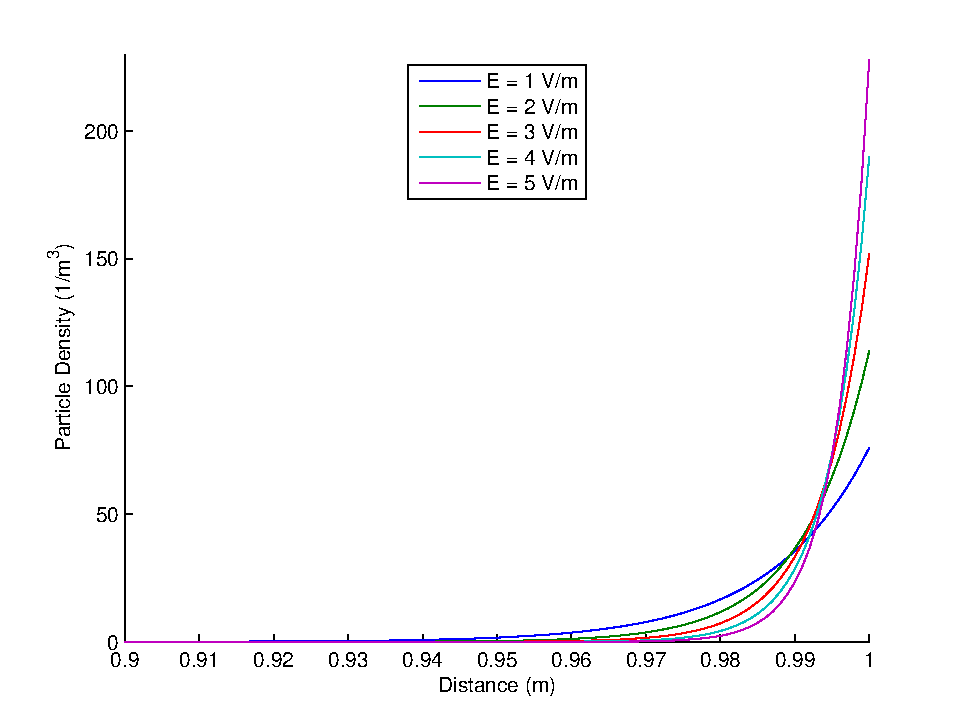
\includegraphics[scale=0.7]{AnalyticSS}
\caption{Increased accumulation of particles due to increased electric field} 
\end{figure}

Debye length is the length over which mobile charge carriers screen out an external electric field and it determines how steeply charges will accumulate over a certain distance. This example also illustrates the decrease in the debye length due to the increase in the charge density. Debye length is determined by the strength of the electric field created by the charge present in the material. The increase in the electric field in this example is analogous to the increase in charge density. Increased charge density creates a larger electric field which pulls a larger amount of charge. This creates a steeper accumulation of the charged particles and a decrease in the debye length. 

\clearpage
\subsection{Transient Solution Over an Infinite Domain}

The problem that will be solved in this section consists of an initial particle density distribution subject to a uniform electric field over an infinitely long conductor. The charge distribution will drift and diffuse over time. This requires a transient solution and the continuity equation (\ref{conn}) needs to be solved. Again, charged particles do not affect the electric field therefore solution of Poisson's equation is not necessary. 

The first step of the solution process is the insertion of \eqref{cdenn} into \eqref{conn}.

\begin{equation}
\frac{\partial n}{\partial t} = \frac{1}{q}\nabla \cdot (\vec{J_n})
\end{equation}


\begin{equation}
\frac{\partial n}{\partial t} = \frac{1}{q}\nabla \cdot (q \mu_{n} n \vec{E}+qD_{n} \frac{dn}{dx} )
\end{equation}

For 1-D this can be simplified to:
\begin{equation}
\frac{\partial n}{\partial t} = \mu_n E \frac{d n}{d x}+D_{n}\frac{d^{2}n}{dx^{2}}
\label{adifg}
\end{equation}

Using separation of variables the solution can be separated into a time and space dependent functions.
\begin{equation}
n(t,x)=n(t)n(x)=n_t n_x
\label{adifn}
\end{equation}
Placing equation \eqref{adifn} into \eqref{adifg} and dividing by n(t,x),
\begin{equation}
\frac{1}{n_{t}}\frac{d n_{t}}{d t}=\mu_n E \frac{1}{n_{x}}\frac{d n_{x}}{dx}+D\frac{1}{n_{x}}\frac{d^2 n_{x}}{dx^2}
\label{Adif}
\end{equation}
Assuming both sides of the equation are equal to a constant -k, time dependent part of the problem becomes a simple first order differential equation.

\begin{equation}
\nonumber
\frac{1}{n_{t}}\frac{d n_{t}}{dl t}=-k
\end{equation}

\begin{equation}
\nonumber
\frac{d n_{t}}{d t}=-kn_t
\end{equation}

Based on the above differential equation $n_t$ can take the following form:

\begin{equation}
n_t=C_1 e^{-kt}
\label{nt}
\end{equation}

Now for $n_x$ assuming a solution of the form below,

\begin{equation}
n_x=C_2 e^{-j\omega x}
\label{nx}
\end{equation}

Placing \eqref{nx} into \eqref{Adif}

\begin{equation}
\omega^2 D C_2 e^{-j\omega x}-j\omega \mu_n E C_2 e^{-j\omega x}+kC_2e^{-j\omega x}=0
\label{omegak}
\end{equation}

Simplifying equation \eqref{omegak} and solving for k gives,

\begin{equation}
k=\omega^2 D+j\omega \mu_n E
\label{k}
\end{equation}

Combining equation \eqref{nt}, \eqref{nx} and \eqref{k} to get the initial form of the solution. $(C=C_1C_2)$

\begin{equation}
n=n_tn_x=Ce^{(-\omega^2 D + j\omega \mu_n E)t} e^{-j\omega x}
\end{equation}

The application of the superposition principle leads to:

\begin{equation}
n=n_tn_x=\int\limits_{-\infty}^{\infty}C(\omega)e^{(-\omega^2 D + j\omega \mu_n E)t} e^{-j\omega x}d\omega
\label{nfinal1}
\end{equation}

The distribution of $n_x$ is known at t=0.

\begin{equation}
n(x,t=0)=\int\limits_{-\infty}^{\infty}C(\omega) e^{-j\omega x}d\omega
\end{equation}

$C(\omega)$ is just the inverse fourier transform of $n(x,0)$.

\begin{equation}
C(\omega)=\int\limits_{-\infty}^{\infty}n(x,0)e^{-j\omega x}dx
\label{comega}
\end{equation}

The final form of the solution is generated by placing equation \eqref{comega} into \eqref{nfinal1}:

\begin{equation}
n=\int\limits_{-\infty}^{\infty}\int\limits_{-\infty}^{\infty}n(z,0)e^{j\omega z}dz e^{(\omega ^2 D-j\omega \mu_n E)t}e^{-j\omega x}d\omega
\label{nfinal2}
\end{equation}

Rearranging equation \eqref{nfinal2},

\begin{equation}
n=\int\limits_{-\infty}^{\infty}\int\limits_{-\infty}^{\infty}n(z,0) e^{(\omega ^2 D-j\omega \mu_n E)t}e^{-j\omega x} e^{j\omega z}  dz d\omega
\end{equation}

Using a gaussian initial distribution results into:

\begin{equation}
n(x,0)=e^{- (\frac{x-x_o}{\sigma})^2}
\end{equation}

\begin{equation}
n(x,t)=\frac{1}{\sqrt{4D_n\sigma^{-2}t+1}}e^{-\frac{(t\mu_n E-x+x_o)^2}{4D_n t+\sigma^2}}
\end{equation}

If the initial distribution is a rectangular then the solution takes the following form:

\begin{equation}
n(x,0)=\prod (w(x))
\end{equation}

\begin{equation}
n(x,t)=\frac{1}{2} erf(\frac{w+2t \mu_n E-2x}{4\sqrt{D_n t}})-\frac{1}{2}erf(\frac{-w+2t \mu_n E-2x}{4\sqrt{D_n t}}) 
\end{equation}

Following plots show the evolution of two particle densities with different initial distributions described above.

\begin{figure}[!htp]
\centering
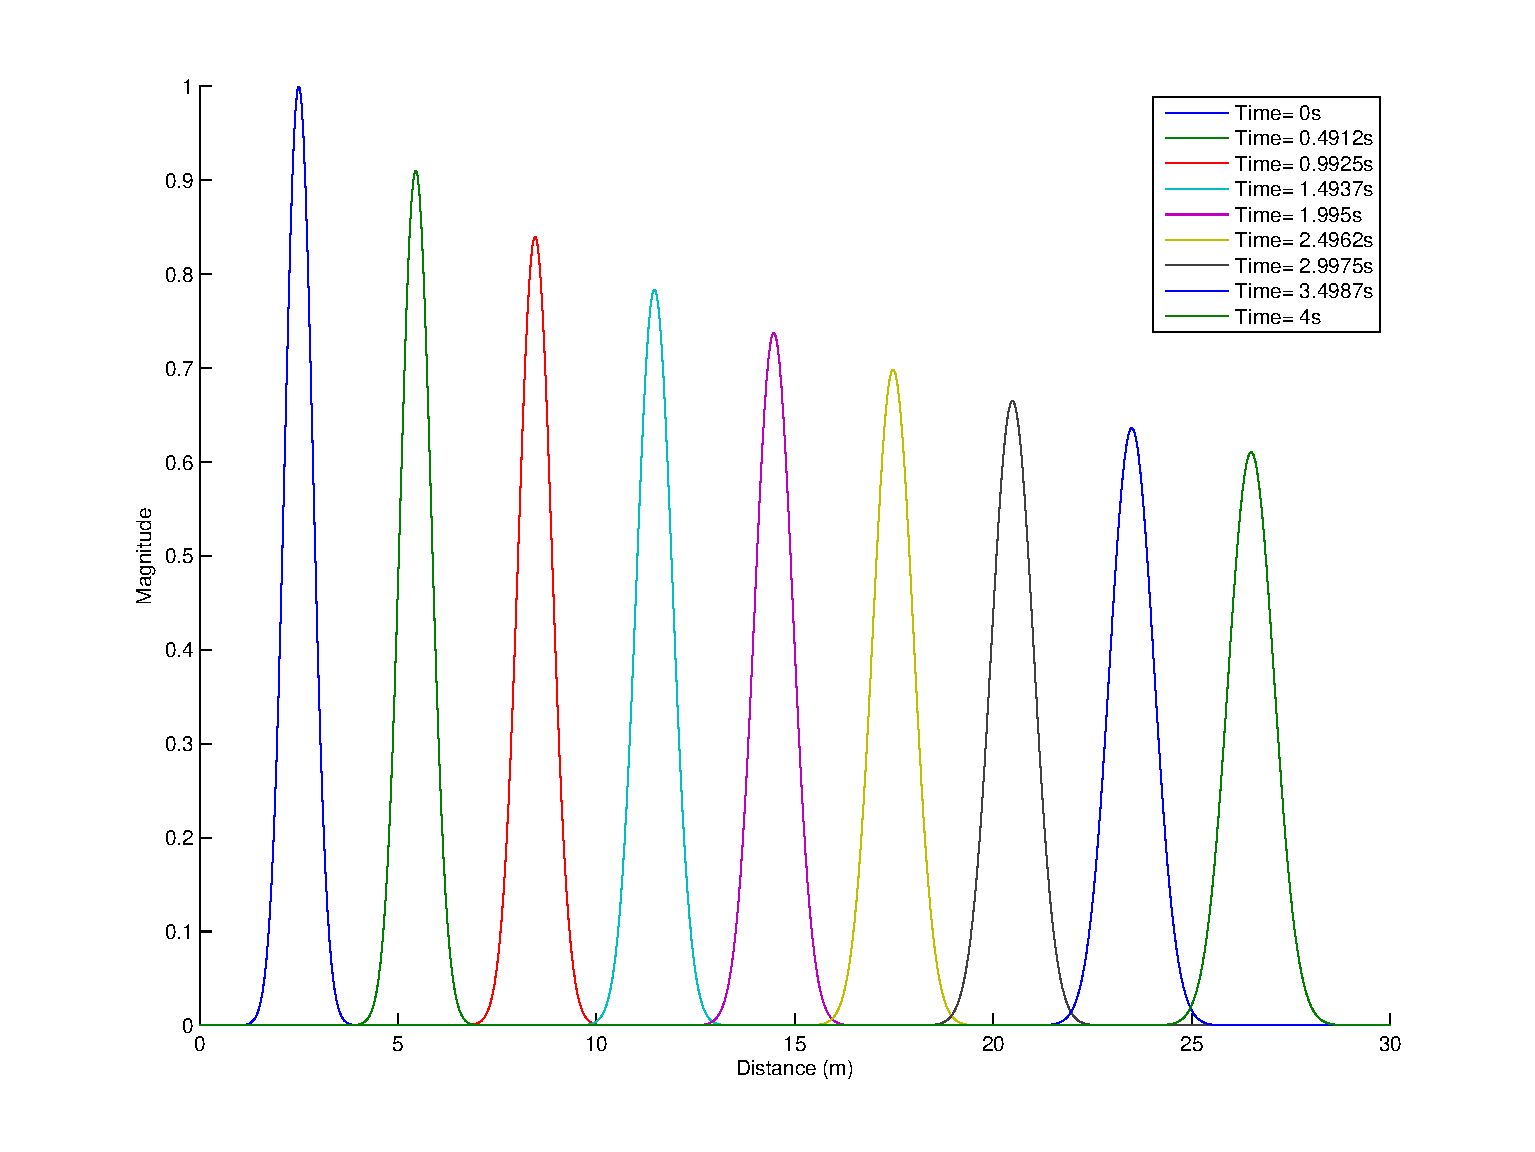
\includegraphics[scale=0.5]{AnalyticGauss}
\caption{A gaussian particle density distribution drifting and diffusion over time} 
\end{figure}

\begin{figure}[!htp]
\centering
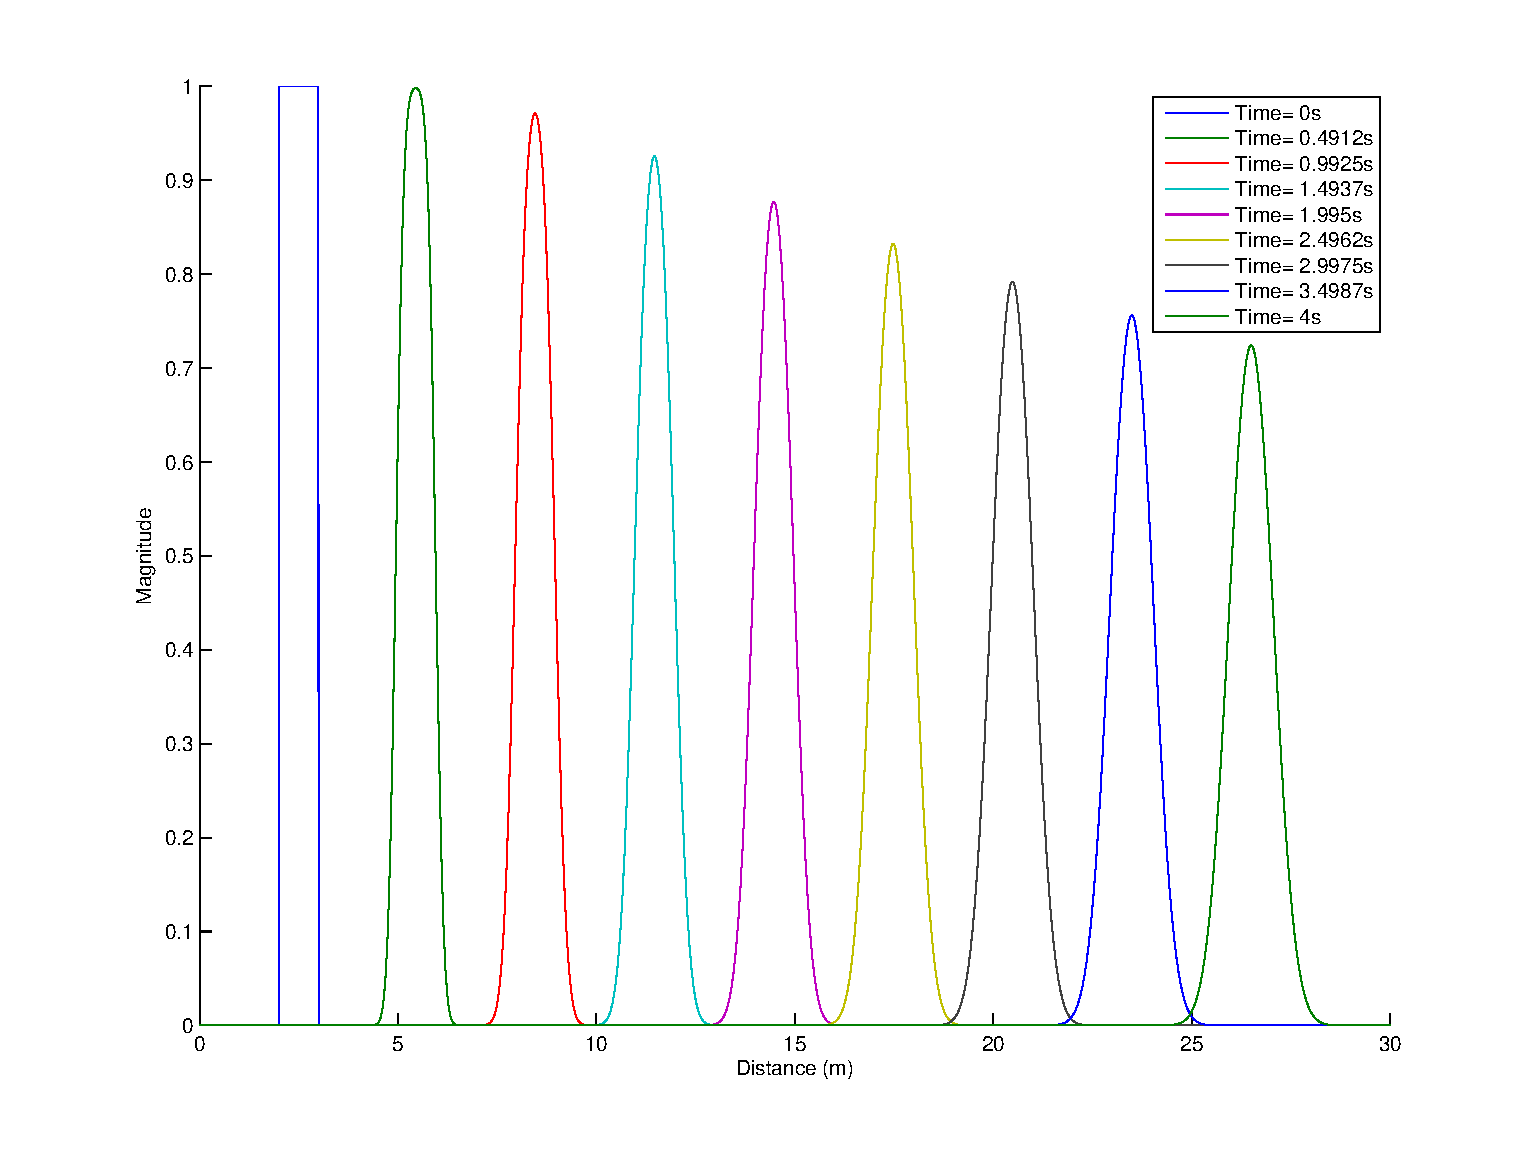
\includegraphics[scale=0.5]{AnalyticRect}
\caption{A gaussian particle density distribution drifting and diffusion over time} 
\end{figure}
\clearpage
\subsection{PN Junction}
Previous analytical solutions involved the solution of Poisson's equation and continuity equation which were not coupled. An example where these equations are tightly coupled will be examined in this section. There are usually no direct analytical solution for coupled equations but it is possible to get a closed form solution by making use of certain approximations. One simple example of this situation is an abrupt p-n junction. An abrupt p-n junction is created when two materials of opposite doping,p type and n type, are brought together. A p type material has an excess number of acceptors $N_A$ and an n type material has an excess number of donors $N_D$. The junction is defined at the interface where $N_A=N_D$. 

\begin{figure}[!htp]
\centering
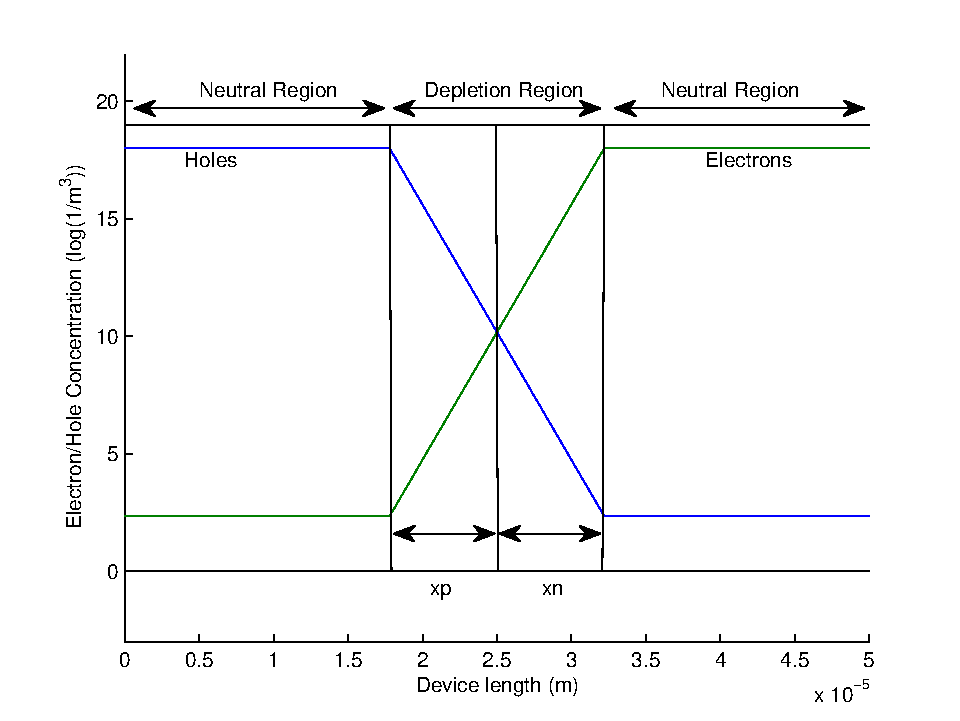
\includegraphics[scale=0.8]{3331}
\caption{PN junction electron/hole density} 
\end{figure}

In this example an analytical solution for an abrupt p-n junction will be derived. To get a solution for this problem depletion region approximation will be used. This approximation starts by assuming that the charges are fully depleted around the junction. All the electric field is confined in the depletion region and regions far away from the junction are neutral. Based on this, the net charge density over the entire region is:

\begin{equation}
\frac{d \vec{E} }{dx}=\frac{\rho}{\varepsilon}=\frac{q}{\varepsilon}(-N_{A}+N_{D})
\end{equation}

\begin{equation}
\rho = \begin{cases}
         0 & \text{for} \;  x<-x_{p}\\
       -qN_{A} & \text{for}  -x_{p}\leq x \leq 0 \\
        qN_{D} & \text{for} \; 0 \leq x \leq< x_{n}  \\
        0 & \text{for}\;  x>x_{n} \\
     \end{cases}
\end{equation}

The electric field over the entire region can be calculated by integrating $\rho$.

\begin{equation}
E = \begin{cases}
       \int \frac{-qN_{A}}{\varepsilon}  dx+ C_{1} & \text{for}  -x_{p}\leq x \leq 0 \\
       \int \frac{qN_{D}}{\varepsilon} dx+ C_{2}   & \text{for } \; 0 \leq x \leq x_{n}  \\
     \end{cases}
\end{equation}

It is possible to solve for $C_{1}$ and $C_{2}$ since electric field must go to zero at $x_{p}$ and $x_{n}$.

\begin{equation}
E(x=-x_{p})=0  \; \;  \Rightarrow  \;\; C_{1}= \frac{-qN_{A}}{\varepsilon}x_{p}
\end{equation}

\begin{equation}
E(x=x_{n})=0  \; \;  \Rightarrow  \;\; C_{1}= \frac{qN_{D}}{\varepsilon}x_{n}
\end{equation}

Then E(x) becomes:

\begin{equation}
E(x) = \begin{cases}
         \frac{-qN_{A}}{\varepsilon}(x+x_{p}) & \text{for}  -x_{p}\leq x \leq 0 \\
         \frac{qN_{D}}{\varepsilon}(x-x_{n})  &  \text{for} \; 0 \leq x \leq x_{n}  \\
     \end{cases}
\end{equation}
 Additionally, the electric field must be continuous across the interface therefore the electric field in the p-type side and the n-type side must equal each other at the interface or when x = 0. 

\begin{equation}
\frac{-qN_{A}}{\varepsilon}(x_{p})=\frac{qN_{D}}{\varepsilon}(-x_{n})
\end{equation}

\begin{equation}
N_{A}x_{p}=N_{D}x_{n}
\label{NAeqND}
\end{equation}This equation makes physical sense since it states that the total charge on one side of the junction must be the same as the total charge on the other. In other words, the net charge on each side keeps the electric field confined to the depletion region.

To find the voltage as a function of distance, equation \ref{Efield} can be integrated.

\begin{equation}
V(x) = \begin{cases}
       \int -E(x)dx=\int \frac{qN_{A}}{\varepsilon}(x+x_{p}) dx = \frac{qN_{A}}{\varepsilon}(\frac{x}{2}+x_{p})+ C_{3} & \text{for}  -x_{p}\leq x \leq 0 \\
       \int -E(x)dx=\int \frac{qN_{D}}{\varepsilon}(x-x_{n}) dx = \frac{qN_{D}}{\varepsilon}(-\frac{x}{2}+x_{n})+ C_{4}  &  \text{for} \; 0 \leq x \leq x_{n}  \\
     \end{cases}
\end{equation}

The potential at one side of the junction can be set to zero. Defining the voltage on the p type side as zero, such that at x= $x_p$, V=0. This gives the constant $C_3$ as:


\begin{equation}
C_{3}=\frac{qN_{A}}{2\varepsilon}x_{p}^{2}
\end{equation}

\begin{equation}
V(x)=\frac{qN_{A}}{2\varepsilon}(x+x_{p})^{2}  \; \; \;\;  \text{for}  -x_{p}\leq x \leq 0 \\
\end{equation}

$C_4$ can be found by using the fact that the potential on the n-type side and p-type side are equal at the interface, such that:

\begin{equation}
V_{p}(x=0)=\frac{qN_{A}}{2\varepsilon}x_{p}^2=V_{n}(x=0)=\frac{qN_{A}}{2\varepsilon}(x_{n}-\frac{x}{2})x+C_{4}
\end{equation}

\begin{equation}
C_{4}=\frac{qN_{A}}{2\varepsilon}x_{p}^2
\end{equation}

Now an overall expression for V(x) can be obtained.

\begin{equation}
V(x) = \begin{cases}
       \frac{qN_{A}}{\varepsilon}(x+x_{p})^2 & \text{for}  -x_{p}\leq x \leq 0 \\
       \frac{qN_{D}}{\varepsilon}(-\frac{x}{2}+x_{n})x  &  \text{for} \; 0 \leq x \leq x_{n}  \\
     \end{cases}
\end{equation}

The maximum voltage across the junction is at  $x= x_{n}$, which is:

\begin{equation}
V_{bi}=\frac{q}{2\varepsilon}(N_{D}x_{n}^2+N_{A}x_{p}^2)
\end{equation}

Using \eqref{NAeqND} in the above equation and rearranging allows $x_{p}$ and $x_{n}$ to be determined. They are:

\begin{equation}
x_{n}=\sqrt{\frac{2\varepsilon V_{bi}}{q}\frac{N_{A}}{N_{D}(N_{D}+N_{A})}}
\end{equation}

\begin{equation}
x_{p}=\sqrt{\frac{2\varepsilon V_{bi}}{q}\frac{N_{D}}{N_{A}(N_{D}+N_{A})}}
\end{equation}

The value of the built in potential can also be calculated using fermi levels of p and n doped materials.

\begin{equation}
E_{FN}-E_{i}=kT \; ln(\frac{N_{D}}{n_i})
\end{equation}

\begin{equation}
E_{i}-E_{FP}=kT \; ln(\frac{N_{A}}{n_i})
\end{equation}
$E_{FN}$ and $E_{FP}$ are fermi energy levels of electrons and holes respectively. The difference between the fermi levels divided by the single electron charge gives us the built in potential of the pn junction.
\begin{equation}
E_{FN}-E_{FP}=q V_{bi}=kT \; ln(\frac{N_{D}}{n_i})+kT \; ln(\frac{N_{A}}{n_i})=kT \; ln(\frac{N_{A}N_{D}}{n_i^2})
\end{equation}

\begin{equation}
V_{bi}=\frac{kT}{q} \; ln(\frac{N_{A}N_{D}}{n_i^2})
\end{equation}

The calculation of the built in potential completes all the necessary equations for the analytical solution of the pn junction without any external bias. Following graphs shows the plots of approximate solutions for net charge, electric field and the junction potential.

\begin{figure}
\centering
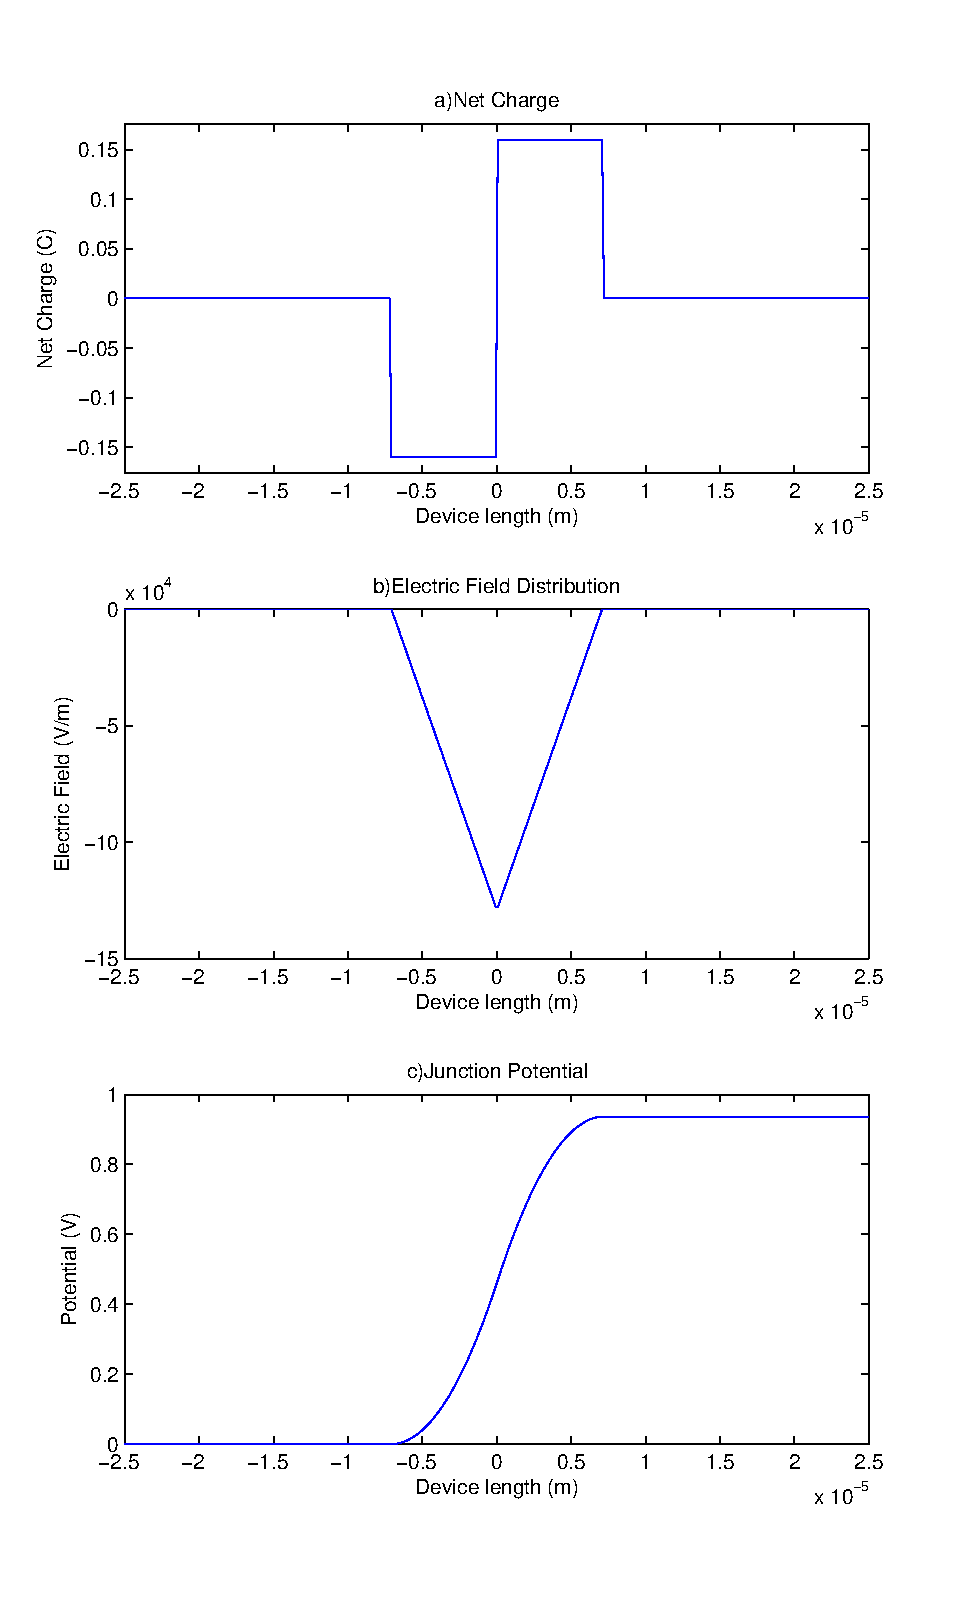
\includegraphics[scale=0.8]{3332}
\caption{Approximate Solution of a PN Junction} 
\end{figure}

\end{doublespace}

